\section{Fazit}

Rückwirkend betrachtet, kann festgehalten werden, dass alle Anforderungen an den Editor gemäß der Projektplanung umgesetzt wurden. Der im Abschnitt \ref{Projektphasen} erwähnte Projektplan konnte eingehalten werden. Die Tabelle in \autoref{fig:sollist} zeigt die tatsächlich benötigten Zeit gegenüber der geplanten. Dabei ist zu erkennen, dass es in den einzelenen Phasen nur zu geringen Zeitabweichungen gekommen ist. Die entstandene Differenzen haben sich untereinander ausgeglichen, wodurch der veranschlagte Zeitrahmen von 70h genau eingehalten werden konnte.

\vfill

\begin{figure}[H] 
	\begin{center}
		\begin{tabularx}{0.90\textwidth}{X|P{50px}|P{50px}|P{50px}}
			\hline \rowcolor{ADITO_RED} \textcolor{white}{\textbf{Vorgang}} & \textcolor{white}{\textbf{Soll}} 								& \textcolor{white}{\textbf{Ist}} 	                            & \textcolor{white}{\textbf{Differenz}} 	\\
			\hline
			1. Analysephase													& 3 h	& 3 h	& 0 h		\\ 
			
			2. Entwurfsphase						 						& 15 h	& 16 h	& + 1 h		\\
			
			3. Implementierungsphase										& 40 h	& 39,5 h& -- 0,5 h	\\
			
			4. Testphase													& 2 h	& 1,5 h	& -- 0,5 h	\\
			5. Dokumentationserstellung										& 10 h 	& 10 h	& 0 h		\\ 
			\hline 
																			& 70 h	& 70 h	& 0 h		\\
		\end{tabularx}
	\end{center}
	\caption{Soll-/Ist-Vergleich} 
	\label{fig:sollist}
\end{figure}

\vfill

Auch das Design konnte wie geplant umgesetzt werden. Vergleicht man den fertigen Editor (\autoref{fig:neuer-editor}) mit dem anfänglich erstellten Designentwurf (\autoref{fig:uxDesigns}) so erkennt man, dass die Anordnung sowie das Aussehen weitestgehend identisch sind.

\vfill

\begin{figure}[H]
	\centering
	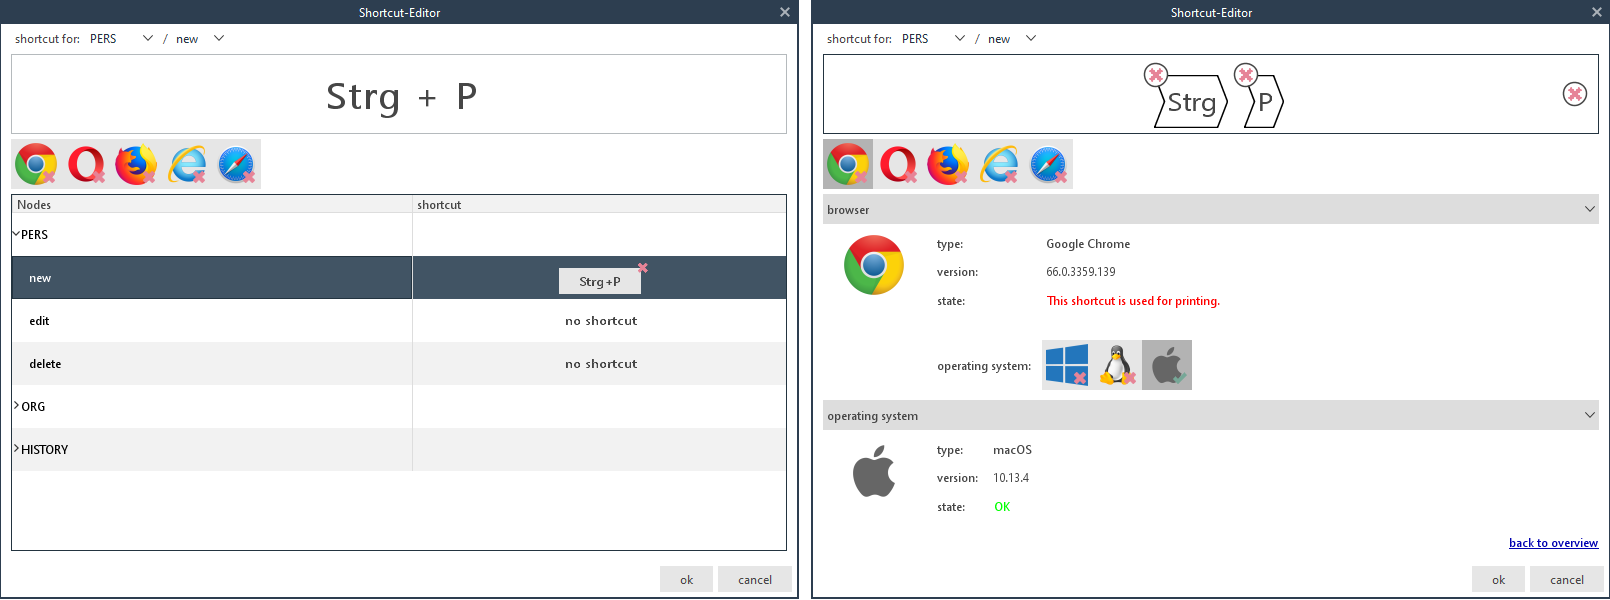
\includegraphics[width=1\linewidth]{../graphic/images/screenshots/Neuer-Editor}
	\caption{Screenshot des Editors}
	\label{fig:neuer-editor}
\end{figure}

\vfill

Da der Editor bisher noch nicht in den ADITO Designer integriert ist, sondern in einer eigenen Umgebung gestartet wird, besteht die zukünftige Aufgabe darin, den Editor an den richtigen Stellen des ADITO Designers einzubinden und die Schnittstellen zu entwickeln. Zudem ist es denkbar, dass in Zukunft zusätzliche Anforderungen an den Editor gestellt werden. Beispielsweise könnte es in Zukunft nötig sein, nach gesetzten Shortcuts suchen zu können.
